\section{Results}
\subsection{Baseline}
For our first set of experiments we wanted to establish a baseline to compare all other results against.  To this end, we created a dataset consisting of approximately 3500 patents.  The samples were evenly split over each of the 7 categoreis with 500 samples per category.  We then trained a support vector machine and a maximum entropy algorithm on the dataset.  The testing accuracy for the support vector machine was
49.33\%, and the testing accuracy for maximum entropy was 46.12\%.  Because there are 7 categories, random chance would put the accuracy at 
14.28\%.  This means that, as a baseline, the algorithms are already performming above random chance.

\begin{figure}[H!]
\centering
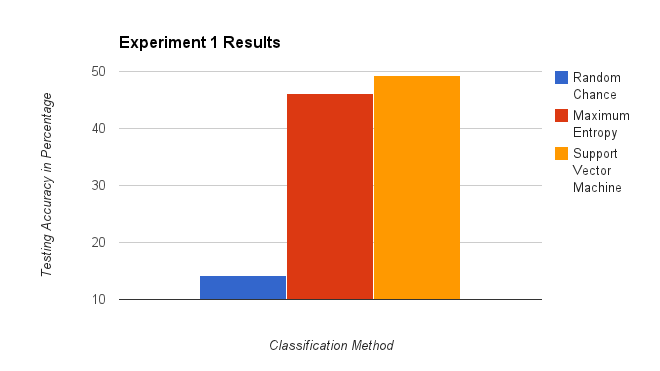
\includegraphics{Experiment Results 1.png}
\caption{Baselines}
\label{overflow}
\end{figure}

\subsection{Dimensionality Reduction}
Due to the large number of features, we first attempted dimensionality reduction on the dataset as a means to increase the accuracy of the algorithm.  To test this, we tried two dimensionality reduction techniques, principle component analysis and laplacian eigenmap.  These dimensionality techiques were applied to the dataset from the baseline analysis.  We found that the results tended to be ambiguous, in that the testing accuracy of maximum entropy tended to increase by approximately 7\% while the support vector machine had its testing accuracy decreased by 7\%.  However, except for these adjustments, the results did not change significantly.
\\
\begin{table}[!Ht]
\caption{Maximum Entropy with Dimensionally Reduction Testing Accuracy}
\centering
\begin{tabular}[!Ht]{| l | l | l |}
\hline
Features & Laplacian Eigenmap & PCA \\ \hline
3 & 14.86\% & 38.86\% \\ \hline
10 & 42.10\% & 50.29\% \\ \hline
50 & 41.90\% &  52.95\% \\ \hline
100 & 42.10\% & 52.00\%	 \\ \hline
1000 & 38.67\% & 45.71\% \\ \hline
\end{tabular}
\end{table}
\begin{table}[H!]
\caption{SVM with Dimensionally Reduction Testing Accuracy}
\centering
\begin{tabular}{| l | l | l |}
\hline
Features & Laplacian Eigenmap & PCA Accuracy \\ \hline
3 & 16.96\% & 18.38\% \\ \hline
10 & 17.81\% & 26.48\% \\ \hline
50 & 26.29\% & 26.19\% \\ \hline
100 & 30.76\% & 32.00 \\ \hline
1000 & 34.57\% & 42.09\% \\ \hline
\end{tabular}
\end{table}
\\ Put in Experiment Results 2 - SVM
\\ Put in Experiment Results 2- Maximum Entropy

\subsection{Dataset Size}
For the third set of experiments we wanted to determine to what extent more data would begin to alter the accuracy the algorithms.  To this end we increased the size of the dataset from 3500 to 20000, and then to 40000 sample patents.  These sample patents were in an identical format to Experiment 1, and no dimensionality reduction was performed on these datasets.  Both the support vector machine and maximum entropy were trained and tested on these datasets.  Overall, the results showed convergence around the 20000 patents for both the support vector machine and maximum entropy.


\begin{table}[Ht]
\caption{Dataset Size and Testing Accuracy}
\centering
\begin{tabular}{| l | l | l |}
\hline
Dataset & Classifier & Testing Accuracy \\ \hline
3500 & SVM & 49.33\% \\ \hline
20000 & SVM & ? \\ \hline
40000 & SVM & 69.53\% \\ \hline
3500 & MaxEnt & 46.12\% \\ \hline
20000 & MaxEnt & ? \\ \hline
40000 & MaxEnt & 69.75\% \\ \hline
\end{tabular}
\end{table}


Insert experiment 3 graph



\subsection{New Features}
For our fourth experiment, we decided to change the type of features collected.  The features were changed by no longer reading from the description of the patent with unigrams, and instead claims and abstract were read and included both unigrams and bigrams. We choose to use a large dataset of 40000 as this sample had a high accuracy in our earlier tests.  The results indicated that the support vector machine had an accuracy of 72.12\% and the maximum entropy algorithm had an accuracy of 72.57\%.  Overall, this is a slight improvement from experiment 3 of 3\% for the support vector machine and an increase of 3\% for the maximum entropy classifier.

\subsection{TfIDF}
Term Frequency
